\documentclass[12,twoside]{article}
\usepackage{lmodern}
\usepackage{amssymb,amsmath}
\usepackage{ifxetex,ifluatex}
\usepackage{fixltx2e} % provides \textsubscript
\ifnum 0\ifxetex 1\fi\ifluatex 1\fi=0 % if pdftex
  \usepackage[T1]{fontenc}
  \usepackage[utf8]{inputenc}
\else % if luatex or xelatex
  \ifxetex
    \usepackage{mathspec}
  \else
    \usepackage{fontspec}
  \fi
  \defaultfontfeatures{Ligatures=TeX,Scale=MatchLowercase}
\fi
% use upquote if available, for straight quotes in verbatim environments
\IfFileExists{upquote.sty}{\usepackage{upquote}}{}
% use microtype if available
\IfFileExists{microtype.sty}{%
\usepackage{microtype}
\UseMicrotypeSet[protrusion]{basicmath} % disable protrusion for tt fonts
}{}
\usepackage[margin=3cm]{geometry}
\usepackage{hyperref}
\PassOptionsToPackage{usenames,dvipsnames}{color} % color is loaded by hyperref
\hypersetup{unicode=true,
            colorlinks=true,
            linkcolor=blue,
            citecolor=blue,
            urlcolor=Blue,
            breaklinks=true}
\urlstyle{same}  % don't use monospace font for urls
\usepackage{graphicx,grffile}
\makeatletter
\def\maxwidth{\ifdim\Gin@nat@width>\linewidth\linewidth\else\Gin@nat@width\fi}
\def\maxheight{\ifdim\Gin@nat@height>\textheight\textheight\else\Gin@nat@height\fi}
\makeatother
% Scale images if necessary, so that they will not overflow the page
% margins by default, and it is still possible to overwrite the defaults
% using explicit options in \includegraphics[width, height, ...]{}
\setkeys{Gin}{width=\maxwidth,height=\maxheight,keepaspectratio}
\IfFileExists{parskip.sty}{%
\usepackage{parskip}
}{% else
\setlength{\parindent}{0pt}
\setlength{\parskip}{6pt plus 2pt minus 1pt}
}
\setlength{\emergencystretch}{3em}  % prevent overfull lines
\providecommand{\tightlist}{%
  \setlength{\itemsep}{0pt}\setlength{\parskip}{0pt}}
\setcounter{secnumdepth}{0}
% Redefines (sub)paragraphs to behave more like sections
\ifx\paragraph\undefined\else
\let\oldparagraph\paragraph
\renewcommand{\paragraph}[1]{\oldparagraph{#1}\mbox{}}
\fi
\ifx\subparagraph\undefined\else
\let\oldsubparagraph\subparagraph
\renewcommand{\subparagraph}[1]{\oldsubparagraph{#1}\mbox{}}
\fi

%%% Use protect on footnotes to avoid problems with footnotes in titles
\let\rmarkdownfootnote\footnote%
\def\footnote{\protect\rmarkdownfootnote}

%%% Change title format to be more compact
\usepackage{titling}

% Create subtitle command for use in maketitle
\newcommand{\subtitle}[1]{
  \posttitle{
    \begin{center}\large#1\end{center}
    }
}

\setlength{\droptitle}{-2em}
  \title{}
  \pretitle{\vspace{\droptitle}}
  \posttitle{}
  \author{}
  \preauthor{}\postauthor{}
  \date{}
  \predate{}\postdate{}

% Colouring links
\usepackage[dvipsnames]{xcolor}
\usepackage{sectsty}
\hypersetup{colorlinks=true, citecolor=blue}

% Spacing
\usepackage{setspace}
\setstretch{1.5}

% Fancy Headers and Footers
\usepackage{fancyhdr}
\pagestyle{fancy}
\fancyhead[OL,ER]{\normalsize R final assigment}
\fancyhead[EL,OR]{\thepage}
\fancyfoot[L]{\small Alvaro Lopez}
\fancyfoot[R]{\small Hertie School of Governance}
\fancyfoot[C]{}
\raggedbottom

\usepackage{rotating}
\usepackage{dcolumn}

\begin{document}

\pagebreak

\pagenumbering{roman} \thispagestyle{empty}

\begin{centering}

\vspace{4 cm}

\Huge

{\bf Final Assigment \\ \Large from Excel to R}

\vspace{1 cm}
{\color{gray} \line(1, 0){250}}
\vspace{2 cm}

\Large
Alvaro Lopez

\normalsize
Master of Public Policy

Class of 2017

\vspace{2 cm}

April 2017

\vspace{3 cm}

\normalsize

\includegraphics[width=.23  \textwidth]{templates/logo.png}

\href{https://www.hertie-school.org/en/}{Hertie School of Governance} 

\end{centering}

\clearpage

\newpage

\thispagestyle{empty} \vspace{4 cm} \small

\normalsize
\clearpage
\newpage
\setcounter{page}{1}

\newpage

\section{Introduction}\label{intro}

The aim of this assignment is to reproduce the data-management work
performed for the MPP master thesis., initially performed in Excel.

The First section describes the data-management work done using R in
order to build a Political Finance Regulation Index, using the IDEA
Political Finance Survey.

In the second section, once calculated, this Index was merged with
several governance variables in order to run a regression analysis for
Latin America.

In the final section, the plots and regression analysis are reproduced
using R.

The text in the following document is a transcription of the master
thesis work, given the aim of this project was reproducing the main
results in R.

\newpage

\thispagestyle{empty} \tableofcontents
\clearpage
\pagebreak

\pagenumbering{arabic}

\section{Methodology}\label{method}

Our aim is to study the relation between control of corruption (the
dependent variable) and political finance regulation (the independent
variable). Following a multivariate model and based on the equilibrium
model by Mungiu-Pippidi (2015) we seek to analyse other independent
variables such as public investment and judicial independence,
considered an opportunity and a constraint of control of corruption,
respectively. Figure I shows a graphical representation of this model.

\begin{figure}[htbp]
\centering
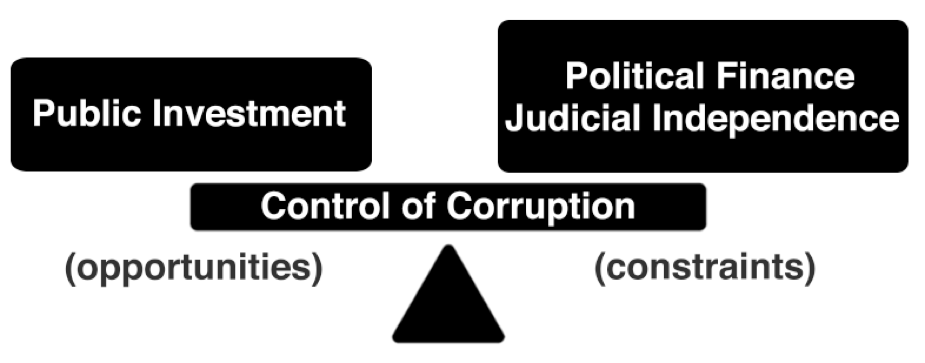
\includegraphics{figure_i.png}
\caption{Equilibrium Model}
\end{figure}

To measure the variations of the dependent variable control of
corruption between countries and across time, we decided to use the
index developed by the World Bank for their World Governance Indicators
(WGI). The Control of Corruption (CoC) Indicator of the WGI measures the
extent to which public power is exercised for private gain, including
both petty and grand forms of corruption, as well as capture of the
state by elites and private interests.??? (Kaufmann et al., 2010, p.~4).
The original indicator has a scale of -2.5-2.5 but it was rescaled to
0-10 to avoid negative numbers. With the new scale, 0 is a country with
no control of corruption and 10 is a country with the highest control of
corruption. The WGI has information about more than 200 countries and
goes as far back as 1996.

In the same sense, there was a need for reliable data to analyse one of
the independent variables: political finance regulation. We used the
IDEA Political Finance Database to develop a Political Finance
Regulation (PFR) Index. IDEA includes more than 180 countries and
excludes cases where no elections have been held in the previous 30
years, as well as where political parties are not allowed to exist or
register candidates.

IDEAs Political Finance dataset is comprised of 43 questions, which
reflect each country's legislation in the matter. The database has a
high response rate, with around 7000 answers from more than 1000
sources. In addition, the dataset provides the exact source and year
when the law was enacted on its appendix.

The responses of the IDEA questionnaire are useful to build a
cross-sectional index, but the supplementary information of the legal
sources and documents provides an opportunity to trace changes in the
legislation through the years. With both sources of information, we
built a panel dataset that spans from 1996 to 2015.

Specifically, every YES response in the IDEA questionnaire was coded
with a 1 and every NO with a value of 0. Additionally, a value of 0 was
coded for every previous year of the date that the law in the matter was
enacted, and a value of 1 since that year onwards. It is worth
mentioning that every question taken into account for building the Index
was weighted equally. Also, factor analysis was made to test a different
possible weighting criteria. The correlation between the equal weighted
index and the factor analysis was high.

To build the PFR Index, we considered only YES-NO questions. Because of
this, only 31 questions of the questionnaire where taken into account.
In the case of categorical questions (with different options for a YES
response), the detail of the response was ignored and only filled with a
YES. Qualitative questions in the survey were not taken into account.
Moreover, the answers were divided in the four categories of the
database:

Bans and limits on private income (BLPI), questions 1 to 18. Public
funding (PF), questions 19 to 28. Regulation of spending (RS), questions
29 to 34. Reporting oversight and sanctions (OS), questions 35 to 43.

Following IDEAs criteria, the few cases with sources of judicial
decisions were also taken into account. Additionally, if a question had
legislative sources from different years, the oldest date is considered
as the year the law was enacted. This has the objective of avoiding
favouring specific legislation and to provide methodological simplicity.
In this respect, our indicator was more sensible to older legislation in
questions with multiple sources. Moreover, in questions with only one
source that was updated on a subsequent year, the index takes into
account only the most recent update. Methodologically, this seeks to
provide certainty about the moment when the requirements of that
particular question count as an affirmative answer. This makes the
questions with updated sources more sensible to the most recent
regulation.

The PFR Index is useful for a descriptive analysis of the worlds
legislative efforts of party finance. Also, it provides panel data to do
an inferential statistical analysis of our region of interest, Latin
America, with a model that includes other relevant variables like life
expectancy or percentage of rural population.

For our other independent variable and based on the equilibrium model,
we used data from capital expenditures of Latin American countries
available from the Economic Commission for Latin America and the
Caribbean (ECLAC), a United Nations regional commission to encourage
economic cooperation. This information is provided as a percentage of
GDP of the 20 countries of Latin America. The information as a
percentage does not capture the increase in real terms of these kinds of
expenditures, given the economic growth of the region during this time.
Taking this into account, we multiplied it with information about GDP in
US dollars provided by the World Bank. The ECLAC provides information on
capital expenditure as far back as 2003. Nevertheless, we only used data
from 2006 to 2015 given the limitation on another relevant variable for
our model, judicial independence.

In this study, we also work with a variable developed by the World
Economic Forum (WEF), which measures the independence of the judiciary
from influences of the government, individuals, or companies. (WEF,
2016) This indicator has a scale of 0 to 7, with countries with lower
scores having less judicial independence than countries with higher
scores. This data extends between 2006 and 2015, so a panel data
analysis including this variable would only account for ten yearly
observations for each country. It is worth mentioning that the WEF
Judicial Independence Index excludes Cuba and includes only five years
of observations for Haiti, so our analysis for Latin America excludes
both countries and only takes into account the remaining members of the
ECLAC. Including all of these variables results in an analysis of 18
countries across ten years, or in other words, 180 observations.

The gathered information allows performing a panel data analysis, taking
into account differences between countries as well as changes over time.
We chose to study Latin America because most of its countries have
enacted political finance regulation in the recent years but are still
fighting to increase its levels of control of corruption. Also, all of
the countries in the region are constitutional democracies and have a
common colonial past.

\section{Results}\label{results}

This section includes the results of a descriptive and inferential
statistical analysis of the variables previously mentioned. All of the
figures are based on our calculations and using the aforementioned
databases.

\subsection{The State of Political Finance Regulation in the
World}\label{the-state-of-political-finance-regulation-in-the-world}

The results show an overall incidence of Political Finance Regulation in
most of the countries in the world and a growing trend of efforts in the
matter over the last 20 years. Figure 2 shows the levels of the PFR
Index in 2015. Countries in lighter shades of yellow have lower levels
of regulation; inversely, countries in darker red shades have higher
ones. In the map one can see clearly the high levels of regulation in
Latin America, low levels in Africa and a mixed scenario in Europe and
Asia, considering that there is no data in countries like China and
Saudi Arabia. \pagebreak

\begin{verbatim}
## 180 codes from your data successfully matched countries in the map
## 0 codes from your data failed to match with a country code in the map
## 63 codes from the map weren't represented in your data
\end{verbatim}

\begin{figure}[h]

{\centering 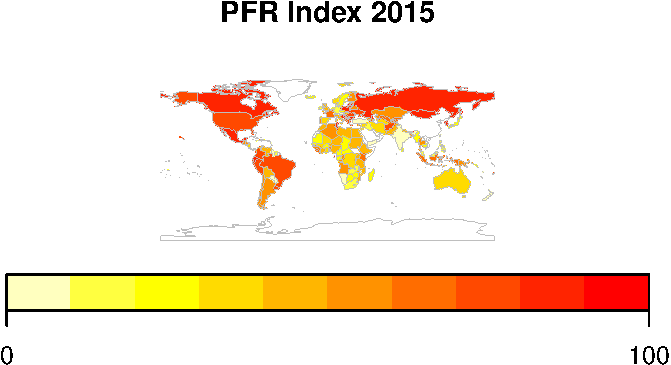
\includegraphics{thesis_body_files/figure-latex/figure_ii-1} 

}

\caption{Worldwide PFR Index, 2015}\label{fig:figure_ii}
\end{figure}

The yearly increase of regulation is evident in Figure 3 which shows the
changes over time of the PFR Index. This figure displays an increasing
trend in the regulation effort in all regions. The slope remains
positive for the period 1996-2005, increasing its steepness after 2006.
Europe is the region that increased its party finance regulation the
most, implementing 55\% of regulations, with notable growth after 2010.
The Americas and Asia occupy the second and third places respectively in
terms of adoption of regulations. \pagebreak

\begin{figure}[h]

{\centering 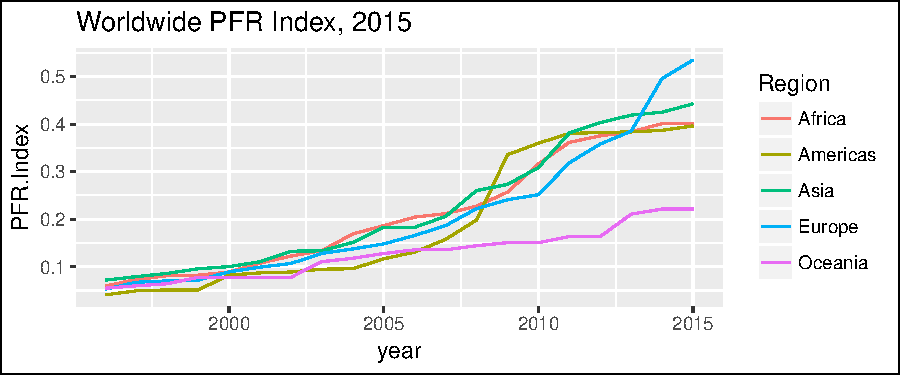
\includegraphics{thesis_body_files/figure-latex/figure_iii-1} 

}

\caption{Worldwide PFR Index, 2015}\label{fig:figure_iii}
\end{figure}

The increase of Party Finance Regulation has not been reflected in
control of corruption. Figure 4 displays the increasing trend of the PFR
Index but also shows that the average of the CoC Indicator has stagnated
and even displays a slight downward trajectory. The evolution of both
suggests that the political finance regulation efforts made by different
countries are not associated with an overall improvement in the control
of corruption. \pagebreak

\begin{figure}[h]

{\centering 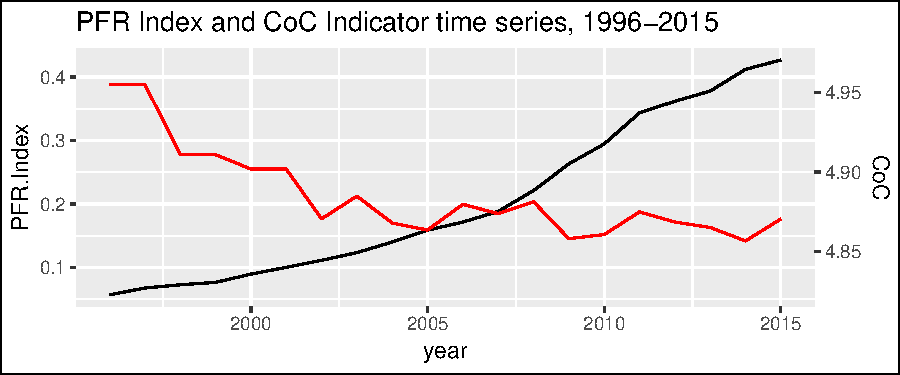
\includegraphics{thesis_body_files/figure-latex/figure_iv-1} 

}

\caption{PFR Index and CoC Indicator time series, 1996-2015}\label{fig:figure_iv}
\end{figure}

The overall increase in the PFR Index is reflected in all the categories
of the database, although there are some small differences to note.
Figure 5 shows that the regulation area that has increased the most in
relative terms in all regions is oversight and sanctions, while the
public funding has been the least regulated issue. Nonetheless, the
figure displays that all the sub-indexes have increased systematically
since 1996. This reflects a widespread trend around the world to
increase Party Finance Regulation in a comprehensive manner, including
regulations across the whole spectrum. \pagebreak

\begin{figure}[h]

{\centering 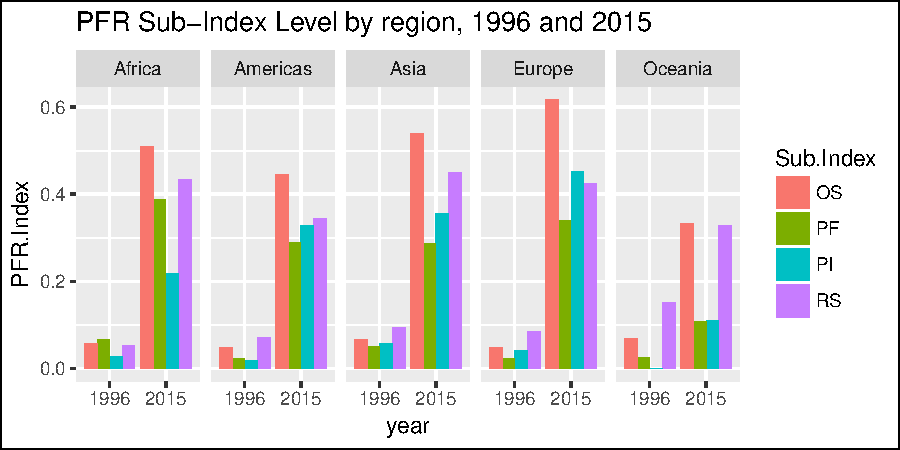
\includegraphics{thesis_body_files/figure-latex/figure_v-1} 

}

\caption{PFR Sub-Index Level by region, 1996 and 2015. BLPI: Bans and limits on private income, PF: Public funding, RS: Regulation on spending, OS: Oversight and sanctions}\label{fig:figure_v}
\end{figure}

\subsection{Political Finance Regulation and Control of Corruption in
Latin
America}\label{political-finance-regulation-and-control-of-corruption-in-latin-america}

The worldwide increase in the PFR Index is also reflected in the Latin
American region. Figure 6 shows that most countries have a medium or a
high degree of PFR. However, there are exceptions like Bolivia,
Venezuela and Paraguay, which show low levels in the PFR Index.
\pagebreak

\begin{verbatim}
## 180 codes from your data successfully matched countries in the map
## 0 codes from your data failed to match with a country code in the map
## 63 codes from the map weren't represented in your data
\end{verbatim}

\begin{figure}[h]

{\centering 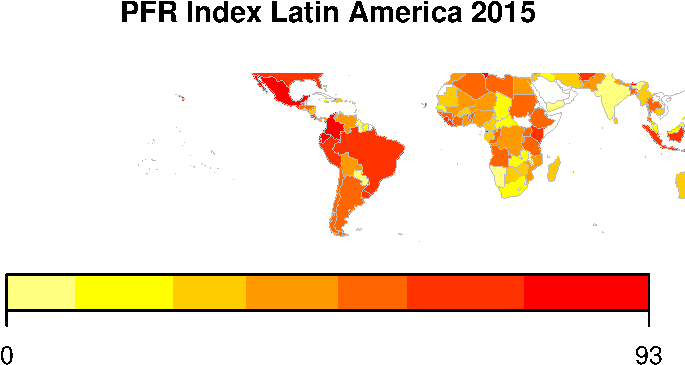
\includegraphics{thesis_body_files/figure-latex/figure_vi-1} 

}

\caption{PFR Index Latin America, 2015}\label{fig:figure_vi}
\end{figure}

Following the worldwide trend, Figure 7 shows the evolution for the PFR
Index and its subcomponents for Latin America. The regulation category
that increased the most is oversight and sanctions. In second place
appears regulation on spending, followed by bans and limits on private
income and public funding. \pagebreak

\begin{figure}[h]

{\centering 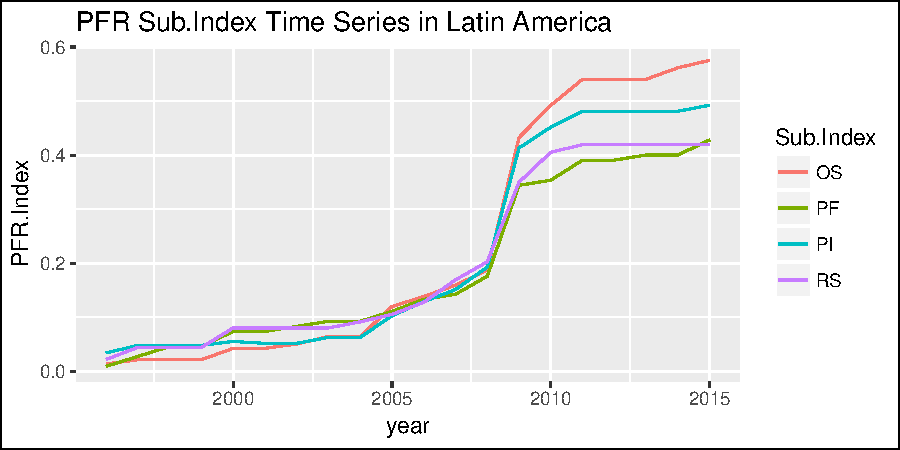
\includegraphics{thesis_body_files/figure-latex/figure_vii-1} 

}

\caption{PFR Sub-index Time Series in Latin America, 1996 to 2015. BLPI: Bans and limits on private income, PF: Public funding, RS: Regulation on spending, OS: Oversight and sanctions}\label{fig:figure_vii}
\end{figure}

Moreover, Figure 8 shows the levels of the PFR Index in 2006 and 2015
for Latin American countries. Results indicate that Ecuador is the
country with the biggest increase in party finance regulation, followed
by Mexico and Colombia. Contrarily, Paraguay and Dominican Republic show
no change. \pagebreak

\begin{figure}[h]

{\centering 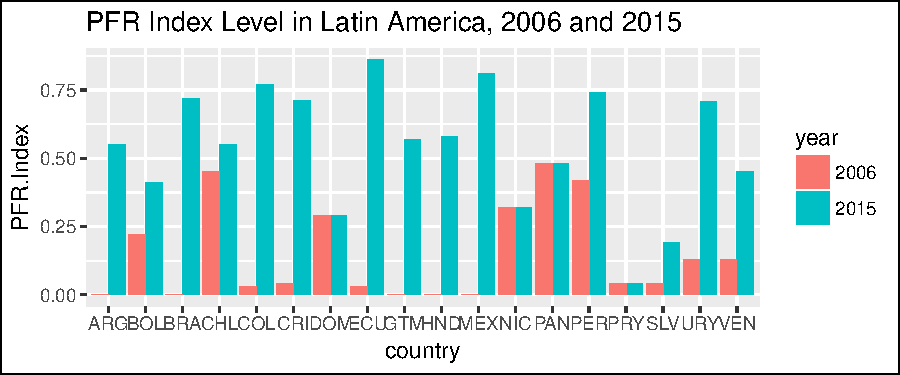
\includegraphics{thesis_body_files/figure-latex/figure_viii-1} 

}

\caption{PFR Index Level in Latin America, 2006 and 2015}\label{fig:figure_viii}
\end{figure}

As with the rest of the world, in Latin America an increase in the PFR
Index is not reflected on the CoC Indicator. Figure 9 shows the average
change in the level of political finance regulation for the region and
the average change of the CoC Indicator from 1996 to 2015. The Figure
also shows that while the CoC Indicator slightly improves for the period
1996-2010 in Latin America, this is reversed after year 2011 with a
strong deterioration of the levels of corruption. \pagebreak

\begin{figure}[h]

{\centering 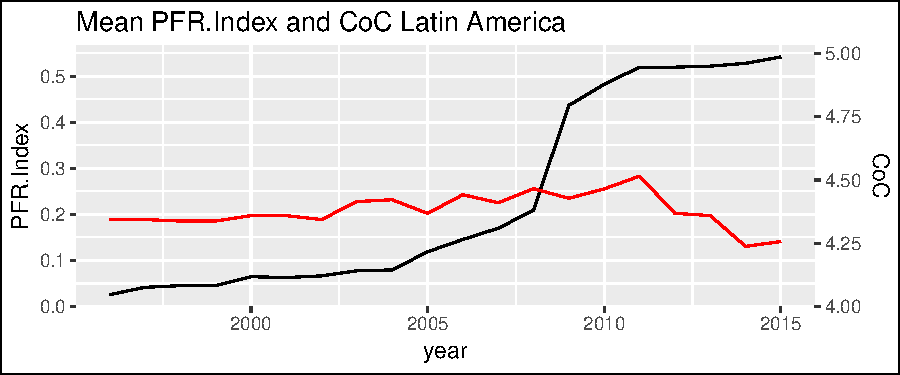
\includegraphics{thesis_body_files/figure-latex/figure_ix-1} 

}

\caption{Mean PFR Index and CoC Indicator series in Latin America, 2006-2015}\label{fig:figure_ix}
\end{figure}

The data shows that countries that increased their regulation the most
between 2006 and 2015 are Ecuador, Mexico and Colombia, which is
represented in Figure 10. This suggests that increases in legislation
are not always correlated with a reduction in the control of corruption.
Ecuador seems to be the exception by showing an improvement in its
control of corruption. In addition, Guatemala, Honduras and Uruguay have
also shown improvements in the last decade. \pagebreak

\begin{figure}[h]

{\centering 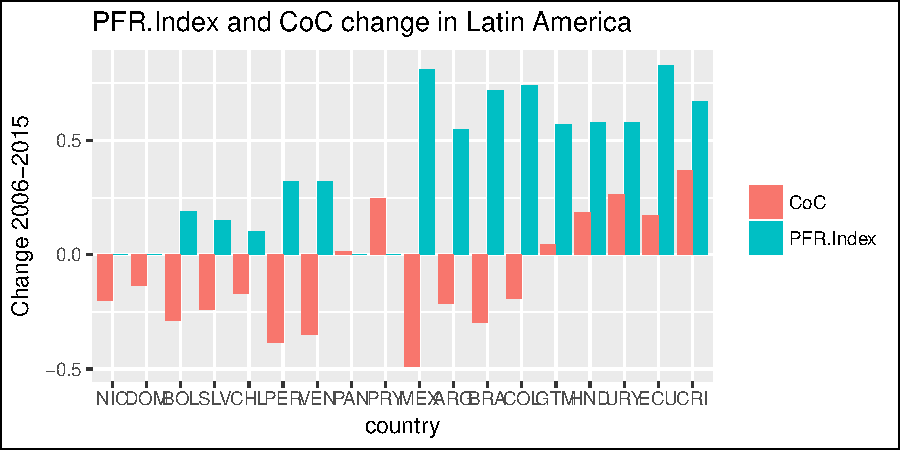
\includegraphics{thesis_body_files/figure-latex/figure_x-1} 

}

\caption{PFR Index and World Bank Control of Corruption Change in Latin America, 2006-2015}\label{fig:figure_x}
\end{figure}

The WEF Judicial Independence Indicator, as illustrated in Figure 10,
complements the relation between control of corruption and political
finance regulation. Among all Latin American countries, there are three
achievers in terms of control of corruption: Chile, Uruguay and Costa
Rica. As seen in Figures 11 and 12, these countries also have the
highest score of judicial independence. Within this group, Uruguay and
Costa Rica made a significant amount of efforts regarding political
finance regulation from 2006 to 2015, while Chiles Index did not rise at
their pace. Also, Uruguay and Costa Rica improved their CoC Indicator,
while Chile??s worsened. This suggests that in countries with high
levels of judicial independence, higher political finance regulation
leads to an increase of control of corruption.\\
\pagebreak

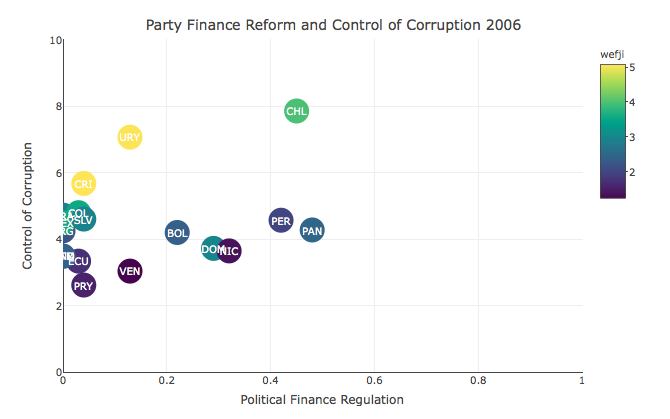
\includegraphics{figure_xi.png} \pagebreak

\begin{figure}[htbp]
\centering
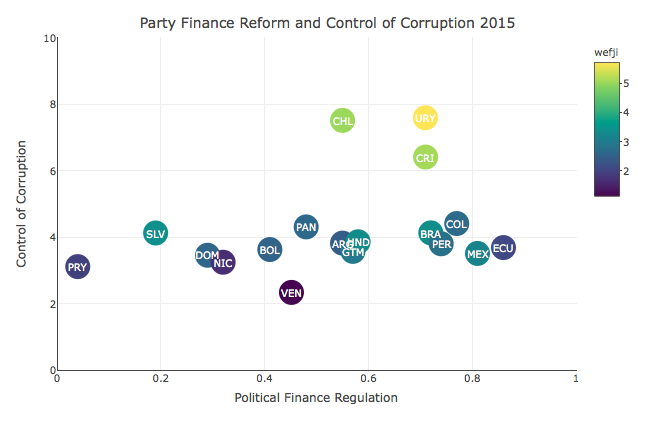
\includegraphics{figure_xii.png}
\caption{Party Finance Regulation and Control of Corruption, 2015}
\end{figure}

\pagebreak

\subsection{Panel Regression Model of Latin
America}\label{panel-regression-model-of-latin-america}

To further explore the relationship between control of corruption,
political finance regulation and judicial independence, inferential
statistics are necessary, allowing to further include other variables
like public investment, as well as control for level of development.
This model includes 18 countries of Latin America from 2006 to 2015.

\subsubsection{Variable Description}\label{variable-description}

As explained in the methodology chapter, the dependent variable is
control of corruption, while the independent variables are political
finance regulation, public investment and judicial independence, using
the previously mentioned indicators. The regression model will
intentionally resemble the equilibrium model described in the
theoretical section of this study. In addition, life expectancy and the
percentage of rural population and are included as control variables for
level of development.

\subsubsection{Multivariate Regression
Model}\label{multivariate-regression-model}

To better reflect the equilibrium model, a multivariate regression is
needed. The multivariate regression model is estimated in equations 1 to
9. Results for pooled OLS, fixed effects (FE) and random effects (RE)
are presented. Several results are offered to assess the robustness of
the analysis.

\begin{equation}
\ CoC_{it} = \beta_{0} +  \beta_{1} PFR_{it} + \beta_{2} PI_{it} + \beta_{3} JI_{it} + \beta{4} JI_{it} PFR_{it} + \beta{5} JI_{it} PI_{it} + RP_{it} + LE_{it} +\epsilon_{it}
\end{equation}

The tables show that increases in political finance regulation are
related with a deterioration of control of corruption in Latin America.
This relationship is statistically significant in the panel estimations.
Inversely, the negative relationship between regulation and control of
corruption becomes positive in countries with high levels of judicial
independence. Furthermore, for countries with high levels of judicial
independence, an increase in political finance regulation has a positive
effect on control of corruption.

\pagebreak

\begin{table}[!htbp] \centering 
  \caption{Panel Regression} 
  \label{} 
\begin{tabular}{@{\extracolsep{5pt}}lcc} 
\\[-1.8ex]\hline 
\hline \\[-1.8ex] 
 & \multicolumn{2}{c}{Control of Corruption} \\ 
\cline{2-3} 
 & Random Effects & Fixed Effects \\ 
\\[-1.8ex] & (1) & (2)\\ 
\hline \\[-1.8ex] 
 PFR & $-$0.295$^{**}$ & $-$0.382$^{**}$ \\ 
  & p = 0.029 & p = 0.019 \\ 
  & & \\ 
 JI & 0.116$^{**}$ & 0.288$^{***}$ \\ 
  & p = 0.016 & p = 0.00000 \\ 
  & & \\ 
 PE & 0.030 & 0.057$^{**}$ \\ 
  & p = 0.155 & p = 0.027 \\ 
  & & \\ 
 PFR*JI & $-$0.099$^{***}$ & $-$0.040$^{**}$ \\ 
  & p = 0.00001 & p = 0.015 \\ 
  & & \\ 
 PFR*PE & $-$0.020$^{**}$ & $-$0.017$^{***}$ \\ 
  & p = 0.038 & p = 0.0003 \\ 
  & & \\ 
 LE & 0.121$^{***}$ & 0.123$^{**}$ \\ 
  & p = 0.007 & p = 0.019 \\ 
  & & \\ 
 RP & $-$0.010 & $-$0.026$^{***}$ \\ 
  & p = 0.177 & p = 0.003 \\ 
  & & \\ 
 Constant &  & 2.341$^{*}$ \\ 
  &  & p = 0.067 \\ 
  & & \\ 
\hline \\[-1.8ex] 
Observations & 178 & 178 \\ 
R$^{2}$ & 0.240 & 0.345 \\ 
Adjusted R$^{2}$ & 0.120 & 0.318 \\ 
F Statistic & 6.884$^{***}$ (df = 7; 153) & 12.781$^{***}$ (df = 7; 170) \\ 
\hline 
\hline \\[-1.8ex] 
\textit{Note:}  & \multicolumn{2}{r}{$^{*}$p$<$0.1; $^{**}$p$<$0.05; $^{***}$p$<$0.01} \\ 
\end{tabular} 
\end{table}

The marginal effects plot in Figure 13 illustrates this relationship,
showing how different levels of the PFR Index and judicial independence
interact with control of corruption, and it uses the following equation:

\begin{equation}
\ frac{\partial CoC_{it}}{\partial PFR_{it}} =  \beta_{1} + \beta{4} JI_{it}
\end{equation}

In brief, efforts in terms of political finance regulation are effective
only in countries with high judicial independence. As Figure XIII shows,
the marginal effect of passing new political finance legislation is
significant when both judicial independence and the PFR Index are high.
Conversely, in countries with low levels of judicial independence,
adding rules to the realm of political finance is self-defeating, since
control of corruption keeps deteriorating.

\begin{figure}[h]

{\centering 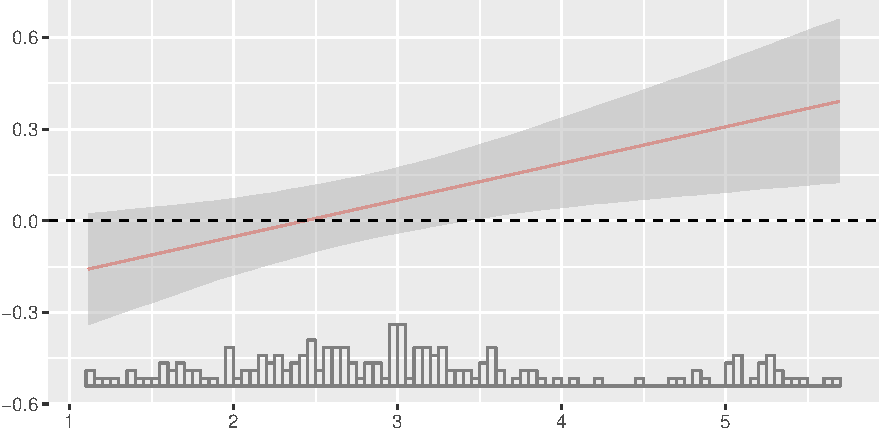
\includegraphics{thesis_body_files/figure-latex/figure_xiii-1} 

}

\caption{Marginal effect of Political Finance Regulation}\label{fig:figure_xiii}
\end{figure}

\section{Conclusions}\label{conclusions}

The main results of the quantitative analysis show that there is a
significant worldwide increase in the levels of political finance
regulation. This trend was also perceived in Latin America. Furthermore,
our statistical model shows that increases in political finance
regulation are related with a deterioration of control of corruption.
This relationship is statistically significant in the panel estimations.
Inversely, the negative relationship between political finance
regulation and control of corruption turns out to be positive in
countries with high levels of judicial independence. In short, for
countries with high levels of judicial independence, an increase in
regulation has a positive effect on control of corruption. In the same
sense, increases in opportunities to corrupt, represented by levels of
public investment, have a significant and negative effect in control of
corruption in countries with lower levels of judicial independence.

\section{Data Management Description}\label{datamanagement}

\subsection{1) PFR\_index}\label{pfr_index}

In this folder is done the datamanagement

\subsubsection{1\_appendix.R}\label{appendix.r}

The IDEA appendix has all of the sources (laws) that were used in order
to answer the survey. The year on which every law was enacted is
extracted. Thus, after running this code, a dataset for every country,
is obtained, on which all of the legal sources are coded with their
respective years. ``Attribution''" is the legal source,
``year\_enforcement'' i the year on which the law was enforced, and
``Temp'' each value temp\_i is the question on which the legal source
was used for every year (Question and question\_i makes more sense
though\ldots{}). The output of this script is
``output\_IDEA\_appendix.csv''.

\begin{figure}[htbp]
\centering
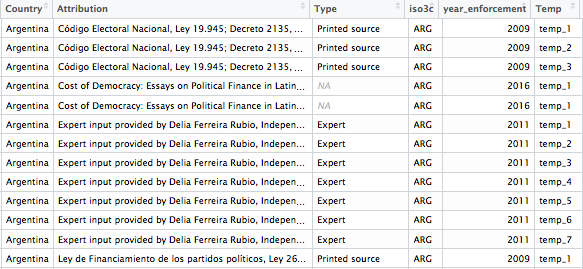
\includegraphics{image_1.png}
\caption{Equilibrium Model}
\end{figure}

\subsubsection{2\_PFRI\_panel.R}\label{pfri_panel.r}

This script builds the following panel dataset, using
``output\_IDEA\_appendix.csv''. ``year\_panel'' is the time dimension of
the panel,which spans from 1925 to 2016. Every country ``iso3c'', has
its set of ``questions'' Ques\_i, for every question the
``year\_enforcement'' is coded, as well as if a ``yes\_no'' answer was
given.

\begin{figure}[htbp]
\centering
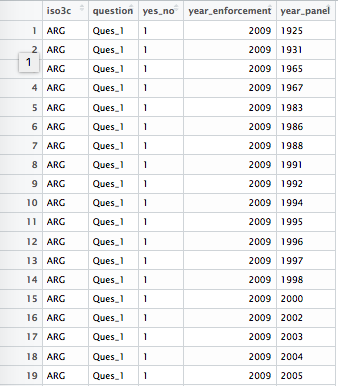
\includegraphics{image_2.png}
\caption{Equilibrium Model}
\end{figure}

\subsubsection{3\_PFRI\_index\_calculation.R}\label{pfri_index_calculation.r}

This script takes the file ``output\_PFR\_Index\_database.csv'' and
calculates the Political Finance regulation Index for every country
using the methodology described above. Thus, takes the simple average
for every question for every country across time. Results are in
``output\_panel\_pfr\_index.csv''. PFR\_Index is the Political finance
regulation Index, and the other variables are its sub components.

\begin{figure}[htbp]
\centering
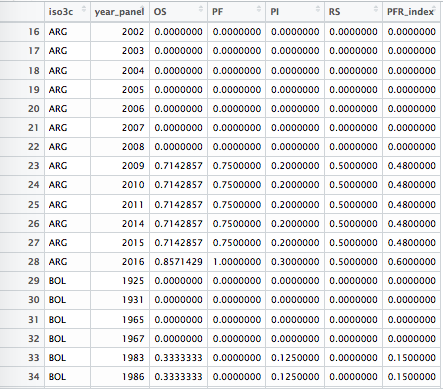
\includegraphics{image_3.png}
\caption{Equilibrium Model}
\end{figure}

\subsection{2) DATABASE}\label{database}

The dataset above is merged with the variables used in the model.

\subsection{3) FIGURES \& ANALYSiS}\label{figures-analysis}

The datamanagement for figures is done.


\end{document}
